\titleformat{\section}{\normalfont\normalsize\bfseries}{\chaptertitlename\ \thechapter:}{0.5em}{}

\newcommand{\appendixsection}[1] {
    \addtocounter{chapter}{1}
    \addcontentsline{toc}{section}{\chaptertitlename\ \thechapter: #1}
    \section*{\chaptertitlename\ \thechapter: #1}
}

\phantomchapter{Appendices}

\setcounter{chapter}{0}

\appendixsection{Specifications of AFFF}
\begin{figure}[H]
    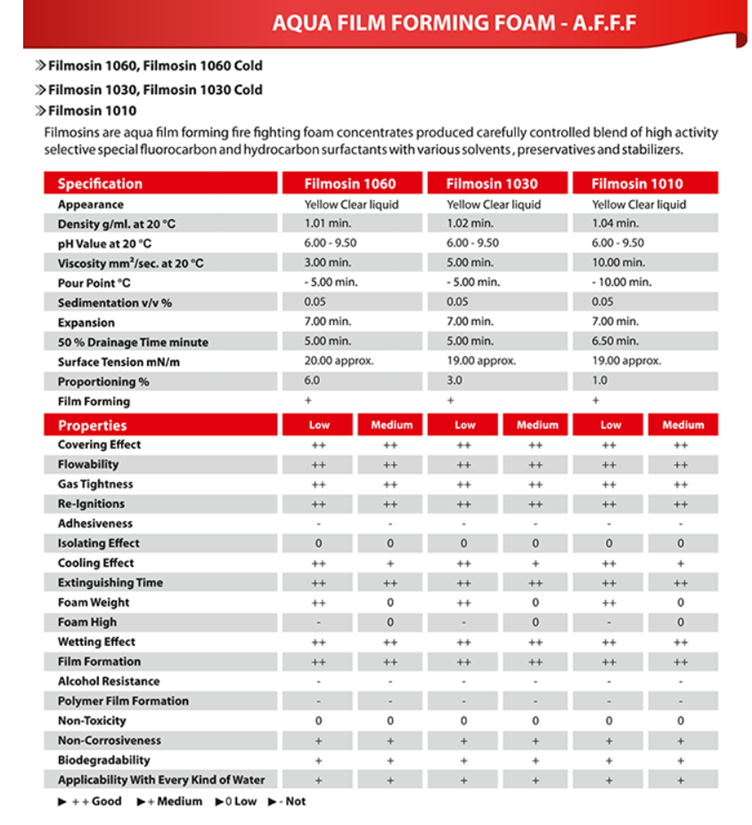
\includegraphics{original_composition_of_afff_concentrate.png}
    \caption{Original composition of AFFF concentrate \cite{hinnant2020characterizing}.}
    \label{appendix:specifications}
\end{figure}

\appendixsection{Properties and specifications of steels}
\begin{figure}[H]
    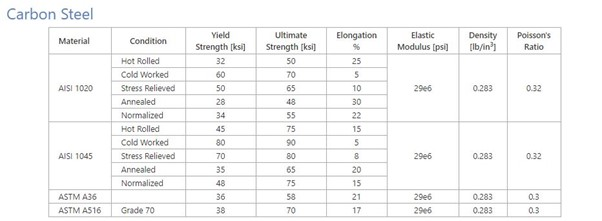
\includegraphics{mechanical_and_physical_properties_of_mild_steel.jpg}
    \caption{Mechanical and physical properties of mild steel (AISI 1020) \cite{kabir2020critical}}
    \label{appendix:carbon_steel_properties}
\end{figure}

\begin{figure}[H]
    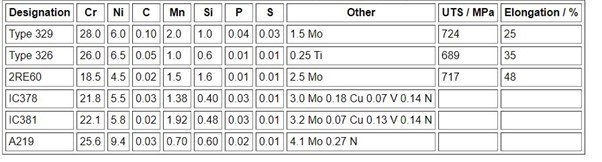
\includegraphics{weighed_composition_of_duplex_stainless_steel.jpg}
    \caption{Weighed composition of duplex stainless steel \cite{sourmail2005stainless}}
    \label{appendix:duplex_stainless_steel_properties}
\end{figure}

\begin{figure}[H]
    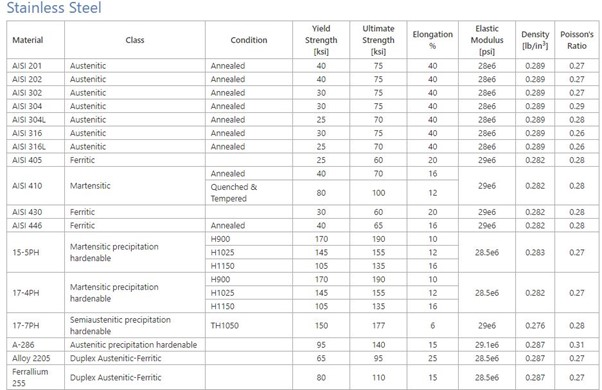
\includegraphics{mechanical_and_physical_properties_of_stainless_steel.jpg}
    \caption{Mechanical and physical properties of stainless steel \cite{bhadeshia2017steels}}
    \label{appendix:stainless_steel_properties}
\end{figure}

\appendixsection{Role of microstructural constituents}

\begin{figure}[H]
\fontsize{10}{12}\selectfont

\renewcommand*{\arraystretch}{1.6}

\begin{tabularx}{\textwidth}{>{\hsize=.6\hsize}X >{\hsize=1.2\hsize}X >{\hsize=1.2\hsize}X}
\hline
Microstructural constituents & Dependent on/characteristics \newline (selection) & Responsible for (examples) \\
\midrule
Vacancies & Temperature, deformation & Hardening at low temperatures; diffusion processes at elevated temperatures; diffusional creep \\
Dislocations & Deformation, temperature, recovery and recrystallization processes; at elevated temperatures edge dislocations may climb, and leave their slip planes & Plastic deformation strength is controlled by their number and motion; driving force for recrystallization; dislocation creep \\
Stacking faults & Crystal structure, alloying & Mobility of dislocations, for example, climb of edge dislocations and cross-slip of screw dislocations is hampered \\
Mechanical twins & Stacking fault energy, deformation, temperature & Additional deformation mechanism at low temperatures and/or high strain rates \\
Subgrains/domains & Deformation, temperature, stacking fault energy/ordered crystal structure; antiphase boundary energy & Work hardening, creep, creation of antiphase boundaries \\
Grain boundaries & Lattice orientation between neighboring grains; subdivision in small-angle, medium-angle and high-angle grain boundaries & Work hardening by acting as barries to slip from one grain to the next; segregation site of impurity atoms \\
Phase boundaries & Alloy system, composition, phase stability at elavated temperatures & Strengthening effects, for example, in duplex or multiphase steels\\
Grains & Alloy system, type of nucleation, processing, deformation, heat treatment, recrytallization & Strengthening (see grain boundaries) but ductility is maintained; grain boundary sliding at elavated temperatures (creep, superplasticity)\\
Annealing twins & Stacking fault energy; characteristic of face-cenntered cubic materials exhibiting a low stacking fault energy & Lowering of total boundary energy during grain growth \\
Precipitates/\newline dispersoids & Alloy system, composition, heat treatment, processing; the interface between particle and matrix can be coherent, semicoherent, or incoherent & Increase in strength by the interaction of moving dislocation; dislocations can loop, cut through or cross-slip the particles at ambient temperatures; at elevated temperatures the dislocations can surmount the particles by climb processes\\
\end{tabularx}

\caption{Role of microstructural constituents on metallic materials \cite{suryanarayana2017microstructure}.}
\label{appendix:role}
\end{figure}

\appendixsection{Full annealing temperature cycle}
\begin{figure}[H]
    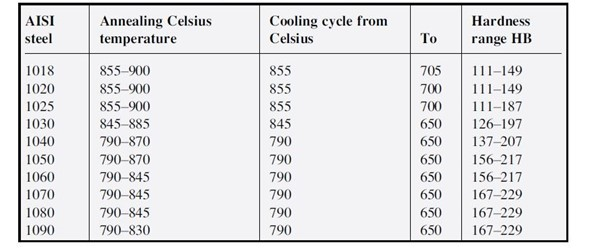
\includegraphics{full_annealing_temperature_cycle.jpg}
    \caption{Full annealing temperature cycle of popular steel and hardness range [66].}
    \label{appendix:range}
\end{figure}

\appendixsection{Effect of changing various substances in PE}
\begin{figure}[H]
    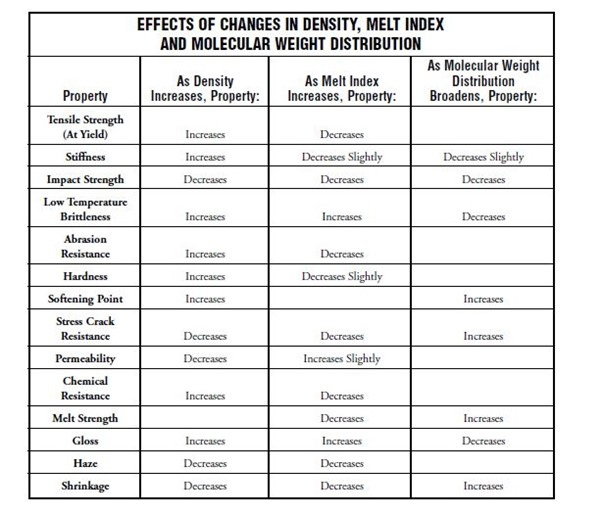
\includegraphics{effect_of_changes_on_properties_of_pe.jpg}
    \caption{The effect of changes in density, melt index, and molecular weight distribution on the properties of PE \cite{gabriel1998history}}
\end{figure}

\begin{figure}[H]
    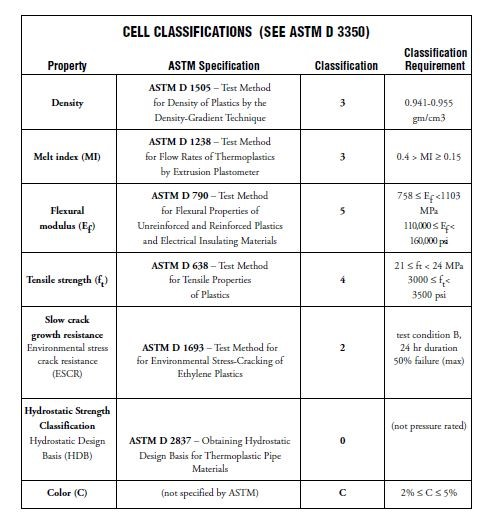
\includegraphics{cell_classifications_for_pe.jpg}
    \caption{Cell classifications for PE \cite{peacock2000handbook}.}
    \label{appendix:classifications}
\end{figure}

\appendixsection{Chemical elements report.}
\begin{figure}[H]
    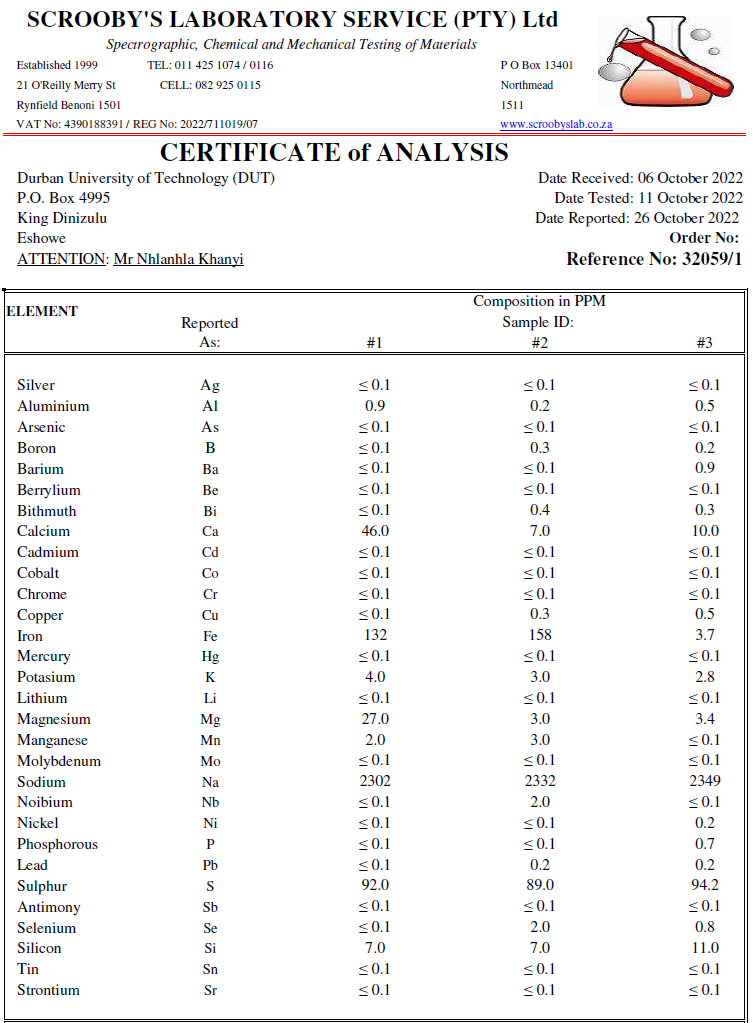
\includegraphics{chemical_elements_of_samples_1-3.png}
    \caption{Chemical elements of samples 1-3}
    \label{appendix:samples_1-3}
\end{figure}

\begin{figure}[H]
    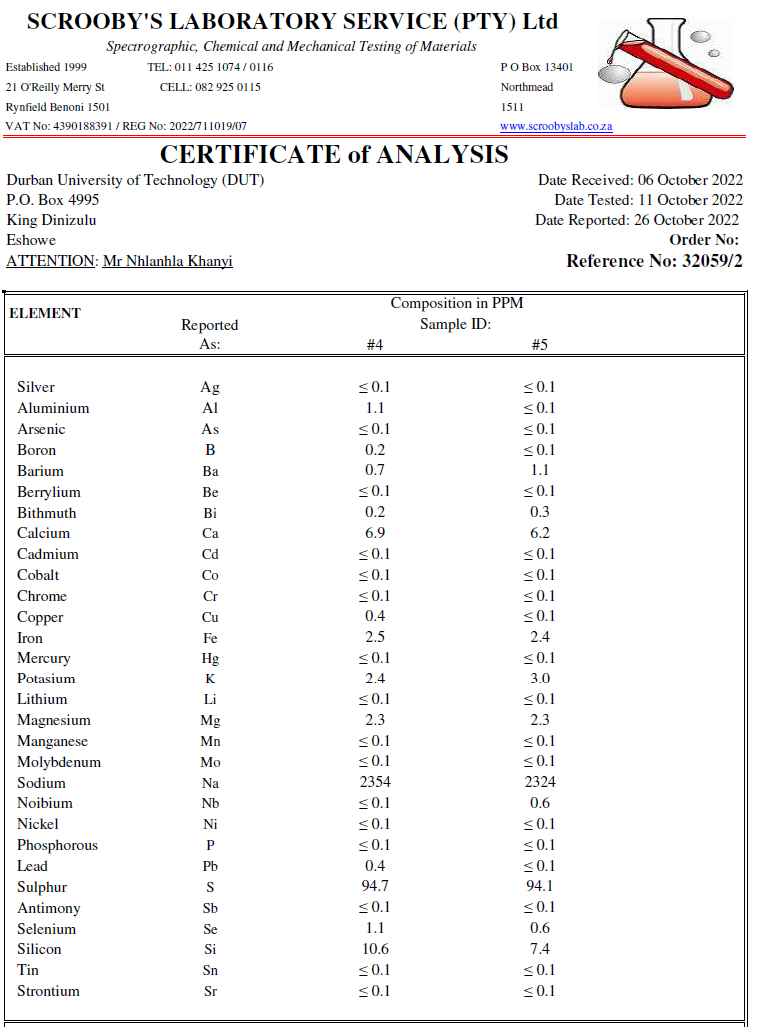
\includegraphics{chemical_elements_of_sample_4.png}
    \caption{Chemical elements of sample 4}
    \label{appendix:sample4}
\end{figure}